\subsection{Descripci\'on del problema}

Somos parte del equipo de desarrollo de una web de ventas de pasajes aereos, y queremos ofrecerles a nuestros clientes un servicio que le calcule el itinerario mediante el cual puede llegar de una ciudad, a otra. Se quiere que el itinerario calculado llegue al destino en el menor tiempo posible. Para esto debe evaluar todos los trasbordos necesarios para que el momento de llegada sea minimo.
Hay una restriccion que dee cumplirse, en un trasbordo, tiene que haber por lo menos dos horas de diferencia entre la hora de llegada a la ciudad, hasta la salida del proximo vuelo. 

\subsection{Resoluci\'on}



%\subsection{Demostraci\'on de la resoluci\'on}


\subsection{Complejidad del algoritmo}


\subsection{C\'odigo fuente}

\lstset{language=C++,
                basicstyle=\ttfamily\footnotesize,
                keywordstyle=\color{blue}\ttfamily,
                stringstyle=\color{red}\ttfamily,
                commentstyle=\color{green}\ttfamily,
                morecomment=[l][\color{magenta}]{\#},
                breaklines=true
}
\begin{lstlisting}


\end{lstlisting}

\subsection{Casos de prueba}

Para este ejercicio escogimos algunos casos de prueba que tienen las siguientes características:

\begin{itemize}

\item Caso sin vuelos hacia la ciudad de destino. En este caso el algoritmo no tiene solucion.
\item Caso con un vuelo directo de origen a destino.
\item Caso con un vuelo directo de origen a destino, pero donde la hora de llegada del vuelo directo es mayor a la hora de llegada tomando una via alternativa.
\item 
\item 

\end{itemize}


\subsection{Performance}



\begin{figure}[H]
\begin{center}
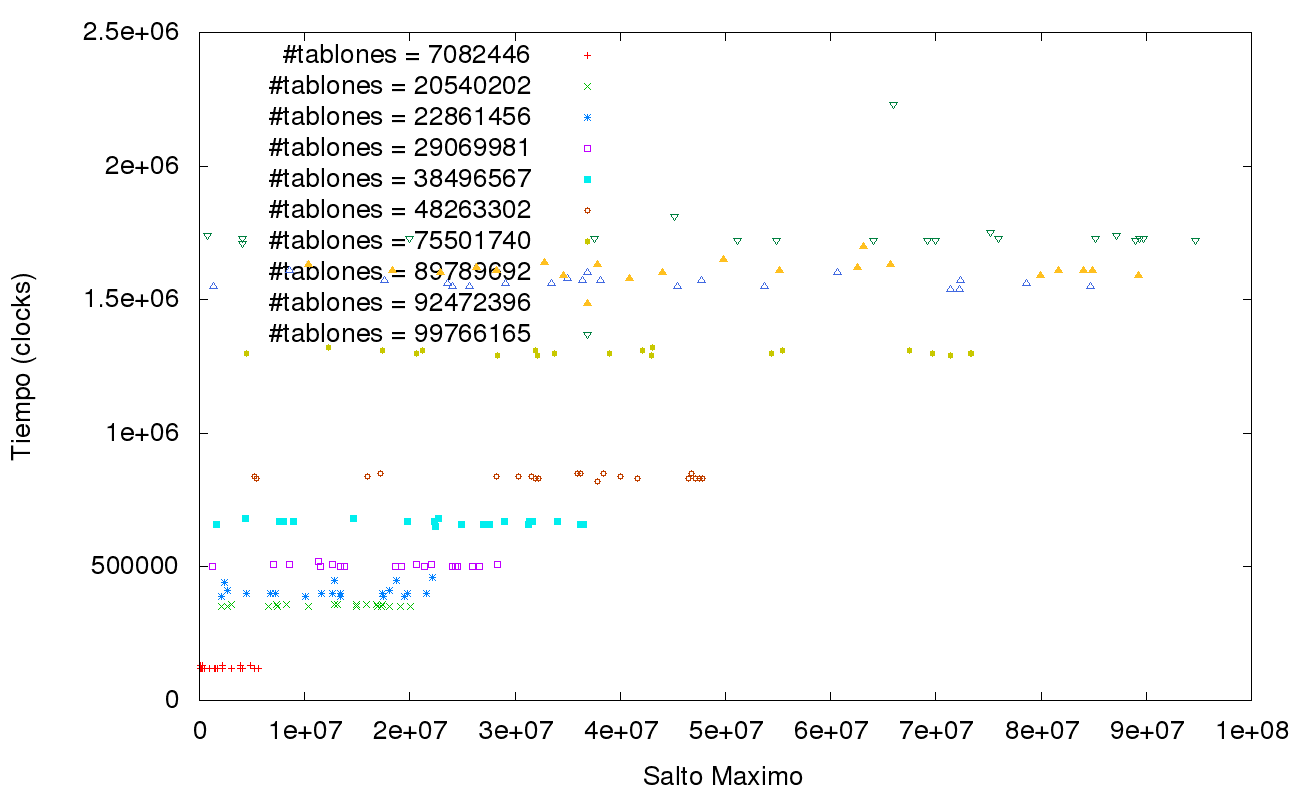
\includegraphics[scale=.45]{./imagenes/ej1_testSaltoMaximo.png}
\caption{Gr\'afico de tiempo en funci\'on del salto m\'aximo.}
\end{center}
\end{figure}

